%\ctparttext{\color{black}\begin{center}
%		Esta es una descripción de la parte de informática.
%\end{center}}

%\part{Parte de informática}
\chapter{Introduction to Quantum Computing}

In this chapter, we aim to provide a general overview to the quantum computing fundamentals required to understand the rest of the thesis. This development will be based on \cite{Nielsen2002}.

\section{Intuitive notions}

\subsection{The Quantum Bit}

The bit is the minimum measure of information on classical computation and classical information theory. Everything in these fields is built from scratch based on bits. Likewise, quantum computing and quantum information theory are built upon the \textbf{qubit}. In this section, we introduce the qubit and its basic properties.

We will describe the qubit as a mathematical object, independent of its physical implementation. By describing them as mathematical entities we will be able to explore their properties mathematically without having to worry about the physics underneath. This lets us construct the quantum computing and quantum information theories independently of the physical implementation. The physical realization of qubits will be briefly discussed on [TODO].

So, what is a qubit? Just like the classical bit, a qubit has a state. For the bit, the two only possible states are either $0$ or $1$. A qubit can take the states $|0\rangle$ and $|1\rangle$ -corresponding to the classical states $0$ and $1$- or it can be in a \emph{linear combination} of them:

$$ |\varphi\rangle = \alpha |0\rangle + \beta |1\rangle $$

Where $\alpha$ and $\beta$ are complex numbers. This is often called \emph{superposition}. The $| \cdot \rangle$ is called the Dirac notation, usually used in quantum physics. So, although we will formalize them later on, we can describe a qubit as a vector in a two-dimensional complex vector space, where $|0\rangle$ and $|1\rangle$ form an orthonormal basis called the \emph{computational basis}. $|0\rangle$ and $|1\rangle$ will be called \emph{computational basis states}.

In classical computation, we may know the state of a bit by consulting it. That is, what can simply retrieve that information from the bit. The first difficulty we find in quantum computing is that once we \emph{measure} a qubit it \emph{collapses} to either $|0\rangle$ with probability $|\alpha|^2$, or to $|1\rangle$ with probability $|\beta|^2$. Thus, $|\alpha|^2 + |\beta|^2 = 1$. The result obtained is gathered \emph{after} the qubit has collapsed to either one of these states, so the outcome may only be either $|0\rangle$ or $|1\rangle$.

The superposition concept might be counter-intuitive, so let us look at them with an analogy. We can think of a coin being tossed as the following qubit:

$$ |\varphi\rangle = \frac{1}{\sqrt{2}} |0\rangle + \frac{1}{\sqrt{2}} |1\rangle $$

This does \textbf{not} represent a coin that has landed somehow on its side, but a spinning coin that has not landed yet. Upon measuring it, we make the coin land and see the result: either heads or tails, and neither of the states in between. This example also describes the qubit collapse: once the coin has landed, we will see the same result every time we look at it -obviously-, just like every time a qubit is measured after the first measurement, the outcome will be the same since it has already collapsed. We will return to this state, which is usually denoted as $|+\rangle$, later on.

Given this behavior, it is worth pointing out that we are not able to find $\alpha$ and $\beta$ by only measuring the qubit due to its collapsing behavior. We can, however, initialize qubits in a certain state and apply some operations to them in order to alter their coefficients, thus knowing their exact value. However, once a single measurement is done, the qubit collapses and the $\alpha$ and $\beta$ values are "lost".

One of the first qubit models ever proposed was the Schrodinger's Cat \cite{Schrodinger1935} \cite{Schrodinger1935a}. In this hypothetical experiment, a cat would be locked in a room for an hour with a device that during that hour would \emph{perhaps} trigger, killing the cat. On the other hand, with equal probability, it would not trigger at all. After the whole hour elapses, the cat would be alive and dead with equal probability, ending up in a halfway state. In this case, our computational bases would be the states alive and dead, and we achieve the state $|+\rangle$ after that hour.

At this point, the reader may ask themselves if a qubit may even physically exist, not just as a mathematical entity. Although we will study qubits mathematically and their physical implementations are discussed in section [TODO: add chapter], we cannot proceed any further without providing a more accurate description of a qubit than a "coin being tossed". A possible realization of qubits is electrons in a single atom's orbit, as seen in Figure \ref{fig 1.1}. An electron in an orbit may be in the so-called \emph{ground} and \emph{excited} states, $|0\rangle$ and $|1\rangle$ respectively, depending on its energy. By shining light to the electron with a certain energy and for a certain amount of time, one can make the electron move from the ground state to the excited state and vice versa. But most interestingly, one can apply the light to the electron during a smaller amount of time, moving the electron somehow "halfway" between both states.


\begin{figure}[h]
	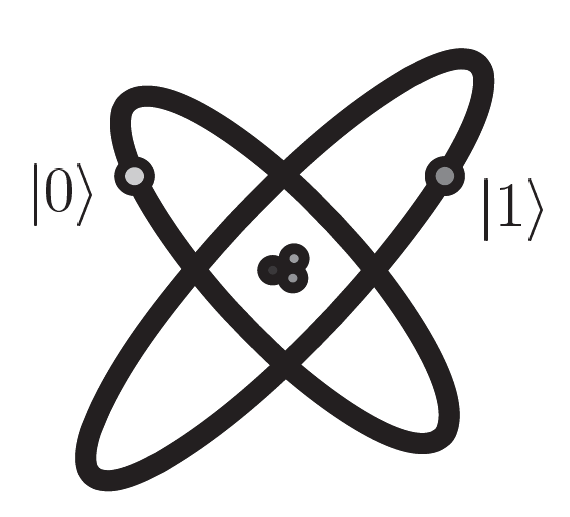
\includegraphics[scale=.4]{../imgs/atom.png}
	\centering
	\caption{Qubit represented by two electron orbits in an atom, \cite{Nielsen2002}.}
	\label{fig 1.1}
\end{figure}

\subsection{Multiple qubits}

Suppose we have a pair of qubits. In the classical case, two bits can be in four possible states: 00, 01, 10, and 11. Similarly, the two qubits computational basis states are $|00\rangle$, $|01\rangle$, $|10\rangle$ and $|11\rangle$. Just like in the single qubit case, our two qubits system may be in a superposition of these four states:

$$ |\varphi\rangle = \alpha_{00} |00\rangle + \alpha_{01} |01\rangle + \alpha_{10} |10\rangle + \alpha_{11} |11\rangle $$

Correspondingly, the measurement of this system will result in either 00, 01, 10 or 11. In fact, it will yield state $x$ with probability $|\alpha_x|^2$, being $\alpha_x$ the coefficient associated with the state $|x\rangle$. The condition of the probabilities adding up to one is called the \emph{normalization condition} and can be expressed as $\sum_{x \in \{0,1\}^2} |\alpha_x|^2 = 1$ for the two qubits case, where $\{0,1\}^2$ are the strings of length two where each character is either $0$ or $1$.

The fundamental differences with the single qubit case start on measurement. Of course, we can measure both qubits at the same time, but we could also measure only one of them. Upon measuring the first qubit we would obtain $0$ with probability $p_0 = |\alpha_{00}|^2 + |\alpha_{01}|^2$, since these are the coefficients associated with the first qubit being $0$. Furthermore, our system will collapse to:

$$ |\varphi'\rangle = \frac{ \alpha_{00} |00\rangle + \alpha_{01} |01\rangle }{ \sqrt{|\alpha_{00}|^2 + |\alpha_{01}|^2} } $$

Note the normalization term $\sqrt{|\alpha_{00}|^2 + |\alpha_{01}|^2}$, applied so the post-measurement state still satisfies the normalization condition. Naturally, after obtaining $0$ in the first qubit we can still obtain either $0$ or $1$ in the second qubit, with probabilities 

$$ \frac{ |\alpha_{00}|^2 }{ |\alpha_{00}|^2 + |\alpha_{01}|^2 }  \ \text{ and } \ 
\frac{ |\alpha_{01}|^2 }{ |\alpha_{00}|^2 + |\alpha_{01}|^2 } $$

respectively, adding up to $1$. Correspondingly, the first qubit being measured will yield $1$ with probability $p_1 = |\alpha_{10}|^2 + |\alpha_{11}|^2$.

Additionally, the first qubit independently should satisfy the normalization condition. That is, its probabilities of being $0$ and $1$ upon measurement must add up to $1$. But those are $p_0$ and $p_1$, which add up to one because of the normalization condition for $|\varphi\rangle$, as expected.

We now introduce the \emph{Bell State} or \emph{EPR pair:}

$$ \frac{ |00\rangle + |11\rangle }{ \sqrt 2 } $$

Although it may seem harmless at first glance, this state has been responsible for many surprises during the development of quantum physics [TODO: reference to the EPR paradox]. Let us have a first look into it, although we will come back to it in section [TODO: añadir referencia a la seccion dodne comentamos el problema de la teletransportación cuántica].

Upon measuring this system we may obtain state $|00\rangle$ with probability $1/2$ and state $|11\rangle$ with probability $1/2$. Suppose we measure the first qubit and obtain $0$. Then, the second qubit will always yield $0$ upon measurement. This means both outcomes are \emph{correlated}. This fact is known as \textbf{quantum entanglement}. It rests at the heart of the disparity between classic physics and quantum physics. It was deeply studied first by Einstein, Podolsky, and Rosen (EPR) \cite{Einstein1935} and second by John Bell \cite{Bellt1964}.

Let us finally consider the more general case. In an n-qubits system our computational basis would consist of the sates $|x_1 x_2 \dotsc x_n\rangle$, where $x_i \in \{0,1\}$. As we already know, in a single qubit system we have two amplitudes $\alpha_0$ and $\alpha_1$. We have four amplitudes for a 2-qubits system, eight for a 3-qubits system... And $2^n$ for an n-qubits system. This means that the number of amplitudes grows exponentially as we add qubits to the system. An immense increment concerning the classical case was the quantity of information that our simple holds grows linearly with the numbers of bits. Of course, we already know it is not that simple, since there are huge limitations on how we may access this information in the quantum realm such as how a qubit collapses upon measurement and the non-cloning theorem discussed in section [TODO]. But we can already glimpse the power of quantum computing versus the classical one.

\section{Quantum Mechanics Model}

[SECTION IN PROGRESS]

\subsection{Bra-ket notation and linear algebra preamble}

Let the qubit as a rigorous mathematical construction. As we have already mentioned, a single qubit will be a vector in a complex vector space, but we will need that space to have some extra properties. That is, it will be a projective Hilbert space. Let us review the necessary linear algebra.

Let $V$ be a complex vector space. That is, a vector space over $\mathds{C}$. We will restrict our study to finite complex vector spaces. If $z$ is a vector in $V$, we will denote its coordinates either as $z = (z_1, z_2, \dotsc, z_n)$ or by column notation:

$$ z = 
\begin{pmatrix}
	z_1\\
	z_2 \\
	\dotsc \\
	z_n
\end{pmatrix}
$$

Since $V$ is a vector space we have two basic operations: (vector) addition and scalar multiplication.

In quantum mechanics, the usual notation is the Dirac's, also know \emph{bra-ket} notation. In this context, vectors in a complex vector space are denoted as $|\varphi\rangle$ and are known as \emph{kets}. The only exception to this is the zero vector, which will be denoted as $0 = (0, \dotsc, 0)$ instead of $|0\rangle$ since $|0\rangle$ will be used as something completely different. A \emph{vector subspace} $W$ of $V$ is a subset of $W$ closed for addition and scalar multiplication.

A \emph{base} of a vector space is a set of vectors $|v_1\rangle, \dotsc, |v_n\rangle$ such that they are linearly independent and any given vector $|v\rangle$ can be written as a linear combination of them: $|v\rangle = \sum_{i=1}^n \alpha_i|v_i\rangle$. The \emph{dimension} of a vector space is the number of elements in any of its bases, which is independent from the chosen base.

\subsubsection{Linear operators}

\begin{definition}
	Given two complex vector spaces $V$ and $W$, a \emph{linear operator} is an application $M: V \rightarrow W $ that is linear in its inputs:
	
	$$ M \Big( \alpha |u\rangle + \beta |w\rangle \Big) = \alpha M (|u\rangle) + \beta M (|w\rangle) $$
\end{definition}

If $V$ to $W$ have dimensions $n$ and $m$ respectively, there is a bijection between the operators from $V$ to $W$ and the $n$ by $m$ matrices. Given an operator $M$, the obtained matrix $M'$ is called the \emph{matrix representation} of the linear operator. Furthermore, $M(|u\rangle) = M' \cdot |u\rangle$, so we usually denote the linear operator and its matrix representation by the same letter, and $M(|u\rangle)$ simply as $M|u\rangle$.

We will refer to linear operators simply as \emph{operators}.

\subsubsection{Inner product and Hilbert Spaces}

Lets define another operation within the complex vector spaces.

\begin{definition}
	Let $V$ be a complex vector space. An inner product $\langle \cdot | \cdot \rangle: V^2 \rightarrow \mathds{C}$ is a function such that:
	
	\quad 1) $\langle \cdot | \cdot \rangle$ is sesquilinear. That is,
	
	\qquad 1.1) $\langle \cdot | \cdot \rangle$ is conjugate symmetric: for all $u,v$ in $V$, $\langle u | v \rangle = \overline{\langle v | u \rangle}$.
	
	\qquad 1.2) $\langle \cdot | \cdot \rangle$ is linear on the second variable: for all $u,v,w$ in $V$ and $\alpha, \beta$ in $\mathds{C}$:
	
	$$ \langle u  | \alpha v + \beta w \rangle = \alpha \langle u | v \rangle + \beta \langle u | w \rangle $$
	
	\quad 2) $\langle \cdot | \cdot \rangle$ is definite positive. That is, for all $u$ in $V$, $\langle u | u \rangle \geq 0$ and $\langle u | u \rangle = 0 \Longleftrightarrow v = 0$.
\end{definition}

Given this properties it can easily be proven that $\langle \cdot | \cdot \rangle$ is also conjugate linear on the first variable. That is, for all $u,v,w$ in $V$ and $\alpha, \beta$ in $\mathds{C}$:

$$ \langle \alpha u + \beta v  | w \rangle = \overline{\alpha} \langle u | w \rangle + \overline{\beta} \langle v | w \rangle $$

We will sometimes denote the inner product $\langle \cdot | \cdot \rangle$ as $( \cdot , \cdot )$ to simplify notation.

Two vectors are said to be \emph{orthonormal} if there inner product is zero. We define the norm of a vector $|v\rangle$ by:

$$\parallel |v\rangle \parallel \ = \sqrt{ \langle v|v\rangle }$$

A \emph{unit vector} is a vector $|v\rangle$ such that $\parallel |v\rangle \  \parallel = 0 $. We also say that $|v\rangle$ is \emph{normalized}, and we can normalize any vector except the zero vector by dividing it by its norm.

A base $|v_1\rangle, \dotsc, |v_n\rangle$ is said to be \emph{orthonormal} if every vector is a unit vector and they are pairwise orthogonal. That is, $\langle v_i|v_j\rangle = \delta_{ij}$ where

\[
\delta_{ij} = 
\begin{cases}
	1 & \text{if } i = j  \\
	0 & \text{if } i \neq j
\end{cases}
\]

\begin{definition}
	An \emph{inner product space} is a vector space with an associated inner product. A \textbf{Hilbert Space} is an inner product space that is also complete. space.
\end{definition}

Hausdorff's Theorem states that every finite normed space is complete [TODO: ref Payá], therefore every finite inner product space over $\mathds{C}$ is a Hilbert space. Again, by Hausdorff's theorem we know that every $n$ dimensional Hilbert space is isomorphic to $\mathds{C}^n$. Thus, $\mathds{C}^n$ is the canonical $n$ dimensional Hilbert space and we will focus our study on these spaces.

The canonical inner product in $\mathds{C}^n$ is:

$$ \langle u|v \rangle \ = \sum_{i=1}^n \overline{u_i}v_j $$

where $u = (u_1, \dotsc, u_n)$ and $v = (v_1, \dotsc, v_n)$, for every $u,v$ in $\mathds{C}^n$.

Let $\alpha = a + i \cdot b\in \mathds{C}$. We define the \emph{conjugate}, $\bar \alpha$, as $\bar \alpha = a - i \cdot b$.

\subsubsection{Outer product}

\begin{definition}
	Definition: Let $V, W$ be two vector spaces and $|v\rangle \in V, |w\rangle \in W$. We define the \emph{outer product} between $|v\rangle$ and $|w\rangle$, $|w\rangle\langle v|$, as the only linear operator such that for any $|v'\rangle \in V$, 
	
	$$ (|w\rangle\langle v|) \ |v'\rangle = |w\rangle\langle v|v'\rangle = \langle v|v'\rangle |w\rangle$$
\end{definition}

This identities provide a dual interpretation: the already known product of a complex value $\langle v|v'\rangle$ with a vector $|w\rangle$, and the application of the new operator, the outer product $|w\rangle\langle v|$ to the vector $|v'\rangle$. The outer product is defined so that this duality is held.

Let us consider linear combinations of outer products. By definition, $\sum_i a_i |w_i\rangle\langle v_i|$ is the operator that transforms $|v'\rangle$ into $\sum_i a_i |w_i\rangle\langle v_i|v'\rangle = \sum_i a_i \langle v_i|v'\rangle |w_i\rangle$.

The most important result concerning outer products is the \emph{completeness relation}:

\begin{proposition}[Completeness relation]
	Let $|i\rangle$ be any orthonormal basis of a finite vector space $V$. Then:
	
	$$ \sum_i |i\rangle\langle i | = I $$
\end{proposition}

\begin{proof}
	Let $|v\rangle \in H$. $|v\rangle$ can be expressed as $ \sum_i v_i |i\rangle$ for some complex numbers $v_i$. Notice that $\langle i|v\rangle = v_i$. Therefor:
	
	$$|v\rangle = \sum_i v_i |i\rangle = \sum_i \langle i|v\rangle |i\rangle = \sum_i |i\rangle\langle i|v\rangle = \bigg( \sum_i |i\rangle\langle i|\bigg) |v\rangle$$
	
	Since $|v\rangle$ was arbitrary, proves that $ \sum_i |i\rangle\langle i | = I $.
\end{proof}

\begin{corollary}[Cauchy-Schwarz inequality]
	
\end{corollary}

\begin{proof}
	TODO: To be copied, Box 2.1, page 68, Nielsencheng.
\end{proof}

\subsubsection{Eigenvectors and eigenvalues}

\begin{definition}
	Let $V$ be a vector space and $A$ an operator on $V$. An \emph{eigenvector} is a non zero vector $|v_\lambda\rangle$ such that $A|v_\lambda\rangle = \lambda|v_\lambda\rangle$ for a complex value $\lambda$ called the associated \emph{eigenvalue}.
\end{definition}

Eigenvalues and associated eigenvectors will usually be denoted with the same letter for simplicity: $\lambda$ and $|\lambda\rangle$. We assume the reader is familiar with eigenvectors and values basic notions. For instance, that they may be calculated using the \emph{characteristic equation}: $|I - \lambda A| = 0$.

\begin{definition}
	A \emph{diagonal representation} of an operator $A$ is a representation $\sum_i \lambda_i |\lambda_i\rangle\langle\lambda_i|$ where the $|\lambda_i\rangle$ form an orthonormal set of A's eigenvectors and $\lambda_i$ are the respective eigenvalues. An operator is said to be \emph{diagonalizable} if it allows a diagonal representation.
\end{definition}

\begin{exampleth}
	As an example of this, let us consider the following matrix:
	
	$$ Z = 
	\begin{pmatrix}
		1 & 0 \\
		0 & -1 
	\end{pmatrix}
	$$
	
	This matrix is called the \emph{Z Pauli} matrix. It is relevant for quantum computing and it will be introduced later on along with the rest of the Pauli matrices. For now, lets compute its diagonalizable representation. Since it is already diagonal we can infer that its eigenvalues are $\{1, -1\}$. Computing the diagonal representation we realize that a pair orthonormal eigenvectors are $\{|0\rangle, |1\rangle\}$ respectively. Therefore:
	
	$$ Z = 
	\begin{pmatrix}
		1 & 0 \\
		0 & -1 
	\end{pmatrix} = 
	|0\rangle\langle0| - |1\rangle\langle1|
	$$
\end{exampleth}

A characterization of diagonalizable operators is provided in Theorem (TODO: add reference to spectral decomposition theorem).

\subsubsection{Adjoint and normal operators}

Another way of looking at the inner product is the \emph{adjoint}.

\begin{definition}
	Let $A$ be an operator between $\mathds{C}^n$ and $\mathds{C}^m$, finite dimensional Hilbert spaces. That is, $A \in \mathcal{M}_{n{\times}m}(\mathds{C})$. Then, its \emph{adjoint} or \emph{conjugate transpose} $A^\dagger$ is defined by:
	
	$$ (A^\dagger)_{ij} = \bar A_{ji} $$
\end{definition}

If $|v\rangle$ is a vector, we can compute its adjoint by seeing it as a matrix. By convention, we will denote $|v\rangle^\dagger = \langle v|$. Adjoints of vector are usually called \emph{bras}, making given sense to the \emph{bra-ket} notation since $\langle v| \cdot |v\rangle = \langle v|v\rangle$, where $\cdot$ denotes the dot product.

Some useful algebraic identities associated to adjoints are:

\begin{itemize}
	\item Given an operator $A \in \mathcal{M}_{n}(\mathds{C})$, $A^\dagger$ is the only operator such that for any two vectors $|u\rangle, |v\rangle \in \mathds{C}^n$: $( |u\rangle, A|v\rangle) = ( A^\dagger |u\rangle, |v\rangle)$
	\item For any two operators $A,B$, $(AB)^\dagger = B^\dagger A^\dagger$.
	\item As a corollary, for any vector $|v\rangle$ and for any operator $A$, $(A|v\rangle)^\dagger = \langle v|A^\dagger$.
\end{itemize}

\begin{definition}
	An operator $A$ is said to be \emph{normal} if $AA^\dagger = A^\dagger A$.
\end{definition}

Normal operators have significant relevancy thanks to the following result:

\begin{theorem}[Spectral Decomposition Theorem]
	An operator $A$ is normal if and only if it is diagonalizable.
\end{theorem}
\begin{proof}
	TODO: To be copied, Box 2.2, page 72, Nielsenchen.
\end{proof}

There are two particular cases of normal operators that will be of special interest for us:

\begin{definition}
	An operator $A$ is said to be \emph{Hermitian} if its adjoint is itself: $A^\dagger = A$.
\end{definition}

\begin{definition}
	A matrix $U$ is said to be \emph{unitary} if $UU^\dagger = I$. Similarly, an operator is said to be \emph{unitary} if $UU^\dagger = I$. A unitary operator $U$ also fulfills that $U^\dagger U = I$.
\end{definition}

Clearly, Hermitian and unitary operators are also normal.

\begin{corollary}
	Any Hermitian operator is diagonalizable. Any unitary operator is diagonalizable.
\end{corollary}

The importance of unitary matrices and operators in quantum computing relies on the following

\begin{proposition}
	Unitary operators preserve inner product between vectors. Thus, they also preserve the norm of a vector.
\end{proposition}

\begin{proof}
	Let $|u\rangle, |v\rangle \in \mathds{C}^n$ and $U \in \mathcal{M}_n(\mathds{C})$ be a unitary operator. Then:
	
	$$ ( U|u\rangle, U|v\rangle) = \langle u|U^\dagger U|v\rangle = \langle u|I|v\rangle = \langle u|v\rangle = ( |u\rangle, |v\rangle) $$
	
	Which proves the proposition.
\end{proof}

\subsubsection{Tensor product}






\subsection{Quantum Principles}

El culmen de la parte teorica del trabajo es contar los principios de la cuantica, al menos los tres primeros. Con esto ya entendemos DWave (de hecho absta con el segundo), y podemos pasar a los problemas QUBO.


\subsection{Quantum Gates}

Explicacion de las puertas de único y multiples qubits

\subsection{Quantum Circuits}

Introduccion a los circuitos cuanticos y primeros ejemplos:

- Circuito de copia de un qubit - intimamente relacionado con el teorema de no clonacion, no se si demostrarlo aqui o no.

- Circuito de teletransportacion - este ejemplo es importantisimo porque nos hace entender bien el entanglement y por qué la información no puede viajar a más velocidad que la luz a pesar del entanglement.

\subsection{Quantum algorithms}

Aqui se discuten los primeros algoritmos cuánticos (son ejemplos importantes):

- Paralelismo cuantico: ejemplo sencillisimo que muestra la verdadera potencia de la computación cuantica, con una sola evaluacion de f(x) calculamos el valor de la función para multiples valores a la vez!

- Deutchs

- Deutchs-Jotzsa

- Creo que aqui merece la pena hacer una pequeña introduccion y mencion a los algoritmos mas importantes de la computación cuántica: Grover, transformada cuantica de fourier. Sin entrar en detalles, pero una mención me parece importante. En ese ambito más abtracto quizas merezca la pena realizar la comparacion P vs NP vs BQP, una pincelada y poco más.


\section{Qubit physical realizations}

Esto no tiene por que ser un sección propia, podría ir dentro de alguna de las anteriores, pero creo que estaría bien comentarlo también.


